% ======================================================================
\section{Visión general}
En esta sección se procede al análisis de la interfaz de usuario. Para ello se analizará la interfaz precisa 
para el intérprete y para el cliente runTree.

El intérprete utilizará una interfaz de consola de comandos. Toda la información de salida la presenterá como 
cadenas de carácteres. Así mismo toda la información de entrada la tomará del teclado en formato orden y opciones. 

Por otro lado el cliente runTree presentará una interfaz en la que se disponga de una descripción gráfica de todo el proceso 
de interpretación. Para una descripción del proceso de interpretación se precisa de la visualización del código fuente, un árbol con los nodos
que encierran el significado semántico del código, las distintas tablas de símbolos que referenciarán a varibles, funciones y clases, y una consola
en la que se mostrará información textual.

También un diagrama de navegación en el que se expone las distintas ventanas de la web OMI.
% ======================================================================
\subsection{Intérprete}
El interprete será accesible como cualquier otro comando de la consola del sistema. Este recibirá una serie de opciones y parámetros. 
Las opciones del intérprete tendrán los siguientes propósitos:
\begin{itemize}
\item Determinar cómo se toma el código fuente, pudiéndo ser desde la entrada estándar, un fichero o la propia línea de comandos
\item Ejecutar el intérprete de forma interactiva, mostrando un prompt en el que se introdusca directamente las sentencias
\item Listar y cargar los módulos del intérprete.
\item Ver la ayuda.
\item Abrir un puerto de escucha para peticiones de red.
\item Configurar el formato de la salida que describe el proceso de interpretación.
\end{itemize}

Como cualquier interprete que tome su entrada de la estrada estándar, el interprete OMI puede ser ejecutado por el 
sistema operativo si se indica al comienzo de un script como el shebang del mismo. 
% ======================================================================
\subsection{runTree}
El cliente runTree será accesible desde un navegador web, y presentará una interfaz gráfica compatible con las versiones actuales de estos.
La interfaz gráfica del cliente deberá contener la siguiente información:

\begin{itemize}
\item El código fuente introducido por el usuario y que será enviado a interpretar.
\item El árbol de nodos resultado del análisis léxico y sintáctico. 
\item Las distintas tablas de símbolos que guardarán información sobre las variables, las funciones y las clases que serán creadas.
\item La explicación del proceso semántico llevado a cabo. 
\item La salida producida como fruto de la ejecución del código fuente.
\item La entrada introducida por el usuario y que ha sido solicitada por el código fuente.
\item Información relativa a los nodos y tablas de símbolos que el usuario señale.
\end{itemize}

\subsubsection{Wireframe}
\begin{center}
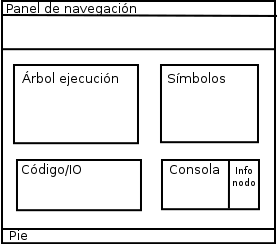
\includegraphics[scale=0.6]{wireframe_runtree.png} \\
\end{center}

\subsection{Sitio web}
El proyecto OMI incluye un sitio web que sirve como presentación del mismo, además de como medio de acceso a la documentación 
y el software desarrollado. Todas las páginas web pertenecientes al sitio contienen información relativa al proyecto y a las áreas que este
ocupa. 

El sitio web OMI se compone de: 

\begin{description}
\item [Página de inicio:] Describe e introduce brevemente el proyecto. Contiene enlaces a las demás secciones del sitio web. Además presenta un
listado de noticias y enlaces de descargas a la última versión del intérprete.
\item [Índice de documentación:] Página que representa un índice de los documentos que conforman el proyecto.
\item [Documentos:] Páginas relativas a la documentación del proyecto en si.
\item [Navegador de clases:] Páginas relativas a la documentación de las clases incluidas en la biblioteca. 
\item [Navegador de ficheros:] Páginas relativas a la documentación de los ficheros que conforman 
el código fuente de la biblioteca y el intérprete.
\item [Navegador de gramática:] Páginas relativas a la documentación gráfica de la gramática del lenguaje.
\item [Descargas:] Página que enlaza la descarga de las distintas versiones del software que conforma el proyecto, disponibles en varios formatos de instalación.
\item [Sobre OMI:] Página con información relativa a la motivación y circunstancias en las que se ha dado el proyecto. Además da detalles sobre los autores y los
organismos implicados en el desarrollo del mismo.
\item [Contacto:] Página con información de contacto.
\end{description}

\subsubsection{Wireframe}
\begin{center}
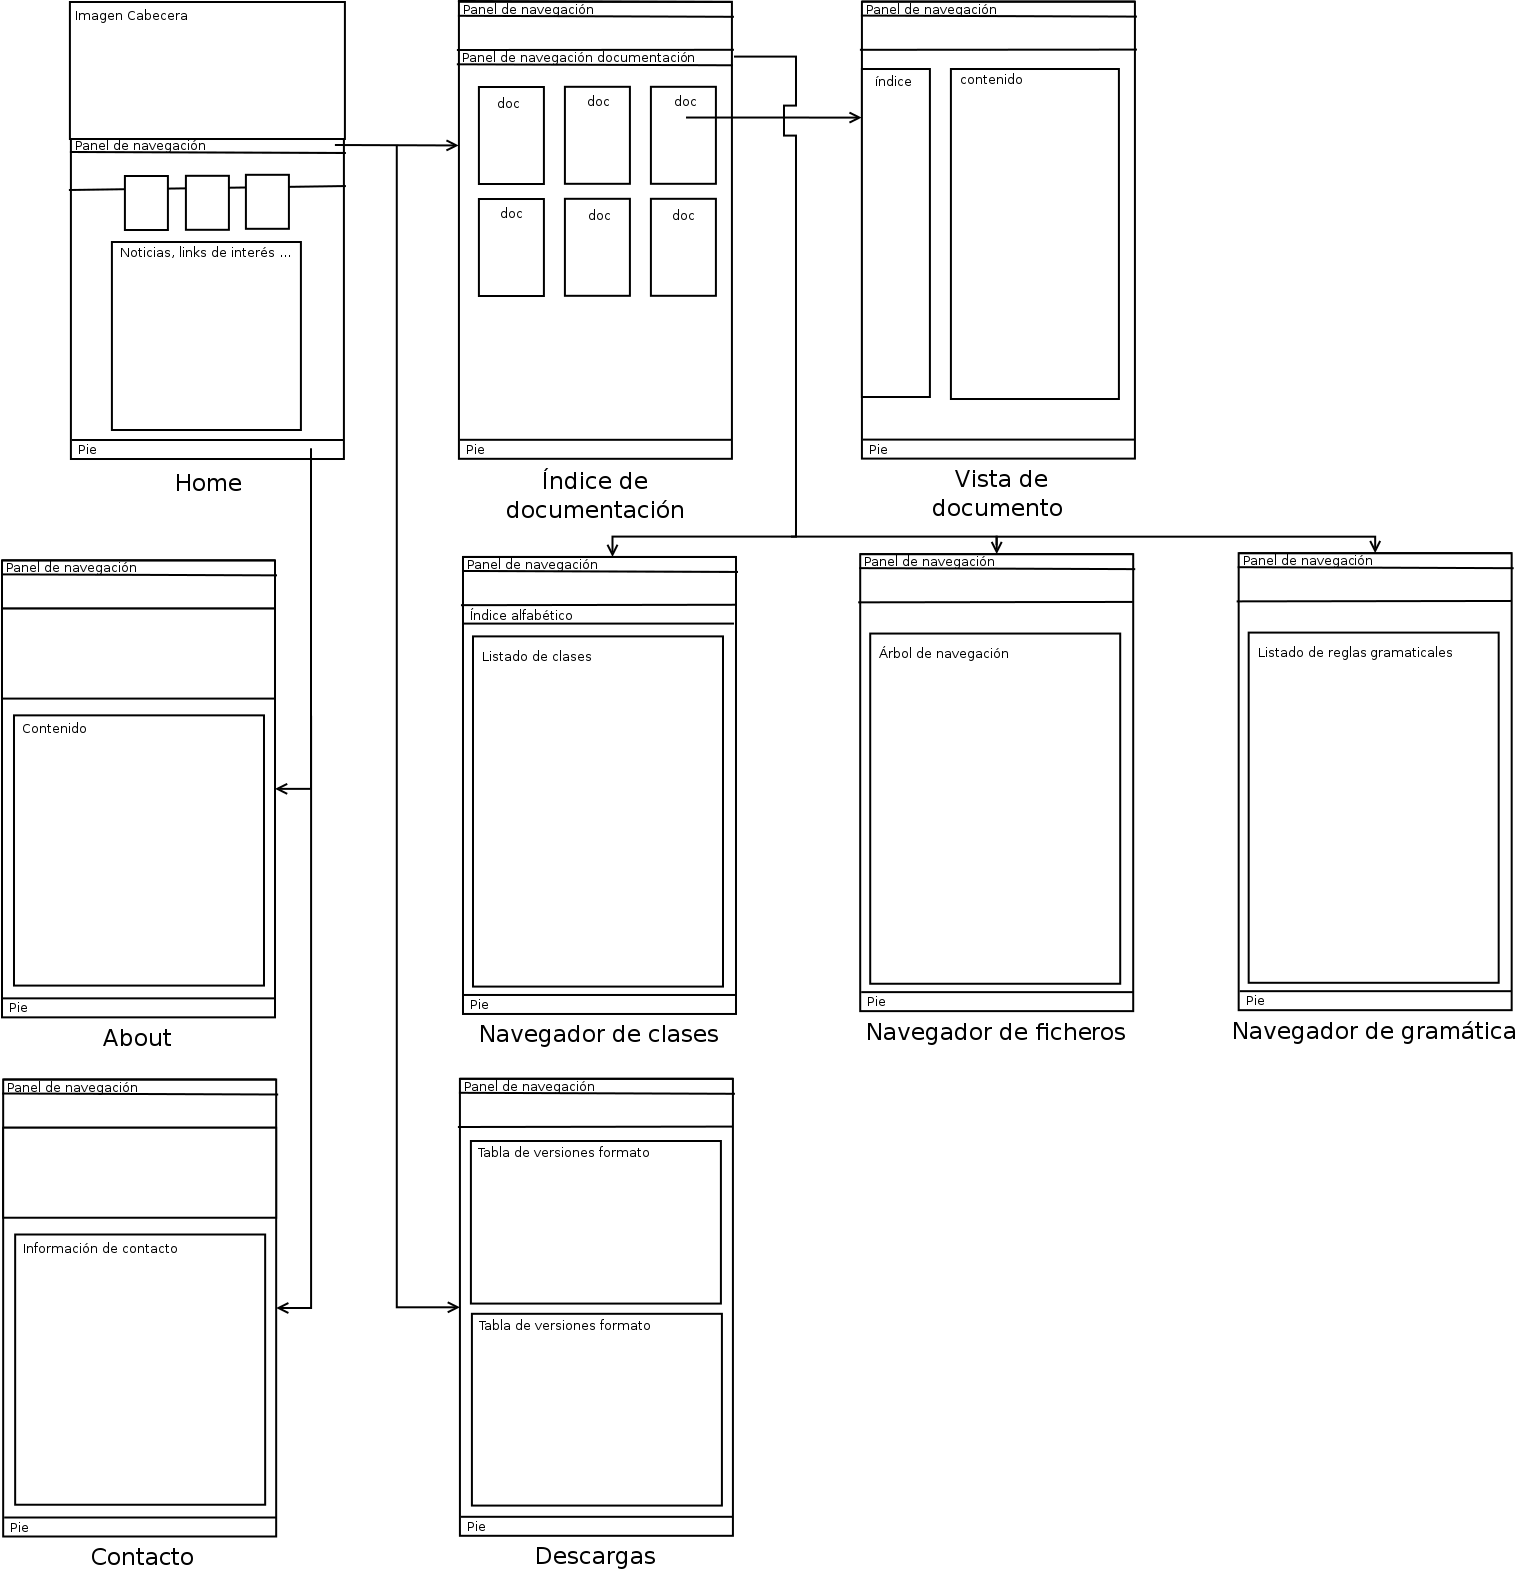
\includegraphics[scale=0.3]{wireframe.png} \\
\end{center}
